\chapter{Finite Elements}
{\color{blue} Ir viendo que algunas cosas de acá van a ir a parar
a Preliminaries.}
\subsection{Definici\'on del \emph{edge element} en prismas} % (fold)
\label{sub:defEdgeElement}
Now we introduce two polynomial spaces which will be used to construct 
the edge elements on the reference prism (Figure~\ref{reference_prism}).
\begin{defi} $R_k(\hat{T})$ is the space of polynomials defined over the
triangle $\hat{T}$ given by
\begin{IEEEeqnarray}{rClCrCl}
    R_k(\hat{T}) & := & P_{k-1}(\hat{T})^2 \oplus S_k(\hat{T}) &\quad&  k&\geqslant&1
\end{IEEEeqnarray}
where
\begin{IEEEeqnarray}{rClCrCl}
    \label{defSk}
    S_k(\hat{T})        & := & \{ \emph{\textbf{p}}\in \tilde{P}_k^2 \,:\;\emph{\textbf{p}}\cdot\emph{\textbf{x}} = 0\}$\quad$\emph{\textbf{x}} & = & (x_1, x_2).
\end{IEEEeqnarray}
\end{defi}
\noindent In order to establish unisolvence we need to calculate
$\dim\left(R_k(\hat{T}) \otimes P_k(\hat{I})\right)$.
\begin{IEEEeqnarray*}{rCl}
    \dim\left(R_k(\hat{T}) \otimes P_k(\hat{I})\right) 
    & = & \dim\left(R_k(\hat{T})\right) \dim\left(P_k(\hat{I})\right) \\
    & = & \dim\left(R_k(\hat{T})\right) (k+1).
\end{IEEEeqnarray*}
\begin{IEEEeqnarray*}{rCl}
    \dim\left(R_k(\hat{T})\right) 
    & = & \dim\left(P_{k-1}(\hat{T})^2 \oplus S_k(\hat{T}) \right)\\
    & = & 2\dim\left(P_{k-1}(\hat{T})\right) + \dim\left(S_k(\hat{T}) \right)\\
    & = & k(k+1) + \dim\left(S_k(\hat{T}) \right).
\end{IEEEeqnarray*}
Para la dimensi\'on de $S_k(\hat{T})$:
\begin{IEEEeqnarray*}{rCl}
S_k(\hat{T}) = \{ \textbf{p} \in \widetilde{P}_k^2 \, : \, \textbf{p}\cdot\textbf{x} = 0 \}.
\end{IEEEeqnarray*}
Consid\'erese
\begin{IEEEeqnarray*}{lll}
    \phi\,:\,\widetilde{P}_k^2 & \longrightarrow & \widetilde{P}_{k+1}\\
    \phi(\textbf{p})    & := & \textbf{p}\cdot\textbf{x}\\
                        & := & x_1p_1 + x_2p_2.
\end{IEEEeqnarray*}
Resulta
\begin{IEEEeqnarray*}{rCl}
    S_k(\hat{T})        & = & \ker(\phi)\\
    \dim(S_k(\hat{T}))  & = & \dim(\widetilde{P}_k^2) - \dim(\img(\phi)).
\end{IEEEeqnarray*}
cualquier $p \in \widetilde{P}_{k+1}$ es
\begin{IEEEeqnarray*}{rCl}
    x_1(a_{k+1,0} x_1^k + a_{k,1} x_1^{k-1}x_2 + \ldots + a_{1,k} x_2^k) + x_2(a_{0,k+1} x_2^k)
        & = & x_1p_1 + x_2p_2
\end{IEEEeqnarray*}
en donde precisamente $p_1$ y $p_2$ pertenecen a $\widetilde{P}_k$, es decir que $\phi$ es
sobreyectiva. Volviendo:
\begin{IEEEeqnarray*}{rCl}
    \dim(S_k(\hat{T}))  & = & \dim(\widetilde{P}_k^2) - \dim(\widetilde{P}_{k+1})\\
                            & = & 2 \dim(\widetilde{P}_k) - \dim(\widetilde{P}_{k+1})\\
                            & = & 2 (k+1) - (k+2)\\
                            & = & k,
\end{IEEEeqnarray*}
entonces
\begin{IEEEeqnarray*}{rCl}
    \dim\left(R_k(\hat{T})\right)   & = & k(k+1) + k\\
                                        & = & k(k+2)
\end{IEEEeqnarray*}
y finalmente
\begin{IEEEeqnarray*}{rCl}
    \dim\left(R_k(\hat{T}) \otimes P_k(\hat{I})\right) 
        & = & k(k+1)(k+2).
\end{IEEEeqnarray*}
($\dim\left(P_K\right) = 3\frac{k(k+1)(k+2)}{2}$).
\begin{defi}\label{edgeelement} Given a natural $k$, the \emph{edge elements}
of degree $k$ are defined by the following:
\begin{enumerate}
    \item $\hat{K}$ is the reference prism $\hat{T} \times \hat{I}$ where $\hat{T} = 
    \{ 0 < x + y < 1 \}$ and $\hat{I} = \{ 0<z<1 \} $.
    \item The polynomial space $P_{\hat{K}}$ is
        \begin{IEEEeqnarray*}{rCl}
            P_{\hat{K}} & = & R_k(\hat{T}) \otimes P_k(\hat{I}) \times 
            P_k(\hat{T}) \otimes P_{k-1}(\hat{I}).
         \end{IEEEeqnarray*} 
    \item The degrees of freedom are:
\begin{IEEEeqnarray}{ll}
    \label{momentos1hcurl} \int\limits_{a} \textbf{u} \cdot \boldsymbol{\tau} \,q\, ds  
        & q\in P_{k-1}\mbox{,} \\
    \IEEEeqnarraymulticol{2}{l}{\nonumber\mbox{ for each edge $a$ with unit tangent } \boldsymbol{\tau} \mbox{;}}\\[8pt]
    \label{momentos2hcurl} \int\limits_{f} \textbf{u} \times \boldsymbol{\nu} \cdot \boldsymbol{q}\,
    d\gamma\mbox{, } &\boldsymbol{q} = (q_1,q_2,0) \in P_{k-2}^2 \times \{ 0 \},\\ 
    \IEEEeqnarraymulticol{2}{l}{\nonumber\mbox{ for each horizontal face $f$ with normal } \boldsymbol{\nu} = (0,0,\pm1) \mbox{;}}\\[8pt]
    \label{momentos3hcurl} \int\limits_{f} \textbf{u} \times \boldsymbol{\nu} \cdot \boldsymbol{q}\,
    d\gamma\mbox{, } &\boldsymbol{q} = (0,q_3,q_2) \in \{ 0 \} \times Q_{k-2,k-1} \times 
    Q_{k-1,k-2}\mbox{, } \\
    \IEEEeqnarraymulticol{2}{l}{\nonumber\mbox{ for the face } f \subseteq \{ x=0 \} \mbox{ with normal }\boldsymbol{\nu} = (-1,0,0) \mbox{;}}\\[8pt]
    \label{momentos4hcurl} \int\limits_{f} \textbf{u} \times \boldsymbol{n} \cdot \boldsymbol{q}\,
    d\gamma\mbox{, } & \boldsymbol{q} = (q_3,0,q_1) \in Q_{k-2,k-1} \times \{ 0 \} \times
    Q_{k-1,k-2},\\
    \IEEEeqnarraymulticol{2}{l}{\nonumber\mbox{ for the face } f \subseteq \{ y=0 \} \mbox{ with normal }\boldsymbol{n} = (0,-1,0) \mbox{;}}\\[8pt]
    \label{momentos5hcurl} \int\limits_{f} \textbf{u} \times \boldsymbol{n} \cdot \boldsymbol{q}\,
    d\gamma\mbox{, } & \boldsymbol{q} = (0,q_3,q_1) \in \{ 0 \} \times Q_{k-2,k-1} \times
    Q_{k-1,k-2}\mbox{, }\\
    \IEEEeqnarraymulticol{2}{l}{\nonumber\mbox{ for the face }f \subseteq \{x+y=1\} \mbox{ with normal }\boldsymbol{n} = (1,1,0) \mbox{;}}\\[8pt]
    \label{momentos6hcurl} \int\limits_{K} \textbf{u} \cdot \boldsymbol{q} \, d\textbf{x}\mbox{, }&\\
    \IEEEeqnarraymulticol{2}{l}{\nonumber q_1, q_2 \in P_{k-2}(x,y) \otimes 
        P_{k-2}(z)\mbox{, }q_3 \in P_{k-3}(x,y) \otimes P_{k-1}(z).}
\end{IEEEeqnarray}
\end{enumerate}
\end{defi}
\noindent{\color{blue}\#\#\#\#\#\#\# poner mas sinteticos los dofs de superficie
aca arriba y aca abajo aclararlos para mostrar como se computan}
In order to clarify how to compute the degrees of
freedom~(\ref{momentos2hcurl})--(\ref{momentos5hcurl}) for an implementation
we write their test spaces more explicitly here.
\begin{IEEEeqnarray}{ll}
    (\ref{momentos2hcurl}) \int\limits_{f} \textbf{u} \times \boldsymbol{\nu} \cdot \boldsymbol{q}\,
    d\gamma\mbox{, } &\boldsymbol{q} = (q_1,q_2,0) \in P_{k-2}^2 \times \{ 0 \},\\ 
    \IEEEeqnarraymulticol{2}{l}{\nonumber\mbox{ for each horizontal face $f$ with normal } \boldsymbol{\nu} = (0,0,\pm1) \mbox{;}}\\[8pt]
    (\ref{momentos3hcurl}) \int\limits_{f} \textbf{u} \times \boldsymbol{\nu} \cdot \boldsymbol{q}\,
    d\gamma\mbox{, } &\boldsymbol{q} = (0,q_3,q_2) \in \{ 0 \} \times Q_{k-2,k-1} \times 
    Q_{k-1,k-2}\mbox{, } \\
    \IEEEeqnarraymulticol{2}{l}{\nonumber\mbox{ for the face } f \subseteq \{ x=0 \} \mbox{ with normal }\boldsymbol{\nu} = (-1,0,0) \mbox{;}}\\[8pt]
    (\ref{momentos4hcurl}) \int\limits_{f} \textbf{u} \times \boldsymbol{n} \cdot \boldsymbol{q}\,
    d\gamma\mbox{, } & \boldsymbol{q} = (q_3,0,q_1) \in Q_{k-2,k-1} \times \{ 0 \} \times
    Q_{k-1,k-2},\\
    \IEEEeqnarraymulticol{2}{l}{\nonumber\mbox{ for the face } f \subseteq \{ y=0 \} \mbox{ with normal }\boldsymbol{n} = (0,-1,0) \mbox{;}}\\[8pt]
    (\ref{momentos5hcurl}) \int\limits_{f} \textbf{u} \times \boldsymbol{n} \cdot \boldsymbol{q}\,
    d\gamma\mbox{, } & \boldsymbol{q} = (0,q_3,q_1) \in \{ 0 \} \times Q_{k-2,k-1} \times
    Q_{k-1,k-2}\mbox{, }\\
    \IEEEeqnarraymulticol{2}{l}{\nonumber\mbox{ for the face }f \subseteq \{x+y=1\} \mbox{ with normal }\boldsymbol{n} = (1,1,0) \mbox{;}}
\end{IEEEeqnarray}
\noindent{\color{blue}\#\#\#\#\#\#\# } 

An illustrative example.
\begin{ejemplo}[edge elements of degree 1]
\begin{IEEEeqnarray*}{rCl}
\hat{\textbf{u}}\,(\hat{x},\hat{y},\hat{z}) &=& 
\left(
    \begin{array}{c}
        a_1 + a_3\hat{y} + a_4\hat{z} + a_6\hat{y}\hat{z} \\[8pt]
        a_2 - a_3\hat{x} + a_5\hat{z} - a_6\hat{x}\hat{z} \\[8pt]
        a_7 + a_8\hat{x} + a_9\hat{y}
    \end{array}
\right)\\[8pt]
(\hat{\textbf{u}}\cdot\boldsymbol{\tau})|_{\boldsymbol{e}}
    &\in&\mathbb{P}_0
\end{IEEEeqnarray*}

\end{ejemplo}

Por la presencia de los momentos~(\ref{momentos1hcurl}) no se puede definir
el interpolador para un campo arbitrario
en $H(\textbf{curl}, K)$, así que por eso to\-ma\-mos co\-mo hi\-pó\-te\-sis
que sea $p>2$ (ver~\cite{monk}, página 134,
~\cite{adams}, Theorem 5.4).
En~\cite{nedelec2} se prueba que este elemento es
$H(\textbf{curl})$--conforme y unisolvente. {\color{BrickRed}>Está
bien usar esta conformidad, siendo que restringimos a Wp?}
\subsection{Definition of the $H(\text{div})$-conforming element on prisms. 
Generalization of the Raviart-Thomas Finite Element} % (fold)
\label{sub:definition_of_the_h_div_element_on_prisms}
With the notation introduced in~(\ref{sub:polynomials}) we consider
the polynomial space
Notaci\'on:{\color{red} Controlar si est\'a bien usada la notaci\'on de prod. tensorial cuando
es un vector de dos coords. por un escalar, y Controlar si es el mismo $h(x,y,z)$ en las coords. 1 y 2 (el 
que es un homog\'eneo en $x,y$ por uno en $z$.)}
\begin{IEEEeqnarray*}{rCl}
    \yesnumber\label{dk}
    D_k & = & P_{k-1}^2(x,y) \oplus \tilde{P}_{k-1}(x,y) \textbf{x},\\
    \textbf{x} & = & (x,y).
\end{IEEEeqnarray*}
\begin{defi}\label{defi_h_div_conforme} The RT element
\begin{itemize}
    \item $\hat{E}$ is the reference prism (Figure~(\ref{reference_prism})).
    \item El espacio $P_{\hat{E}}$ de polinomios es
        \begin{IEEEeqnarray*}{rCl}
            P_{\hat{K}} & = & \{ \boldsymbol{v} = (v_1,v_2,v_3):\,(v_1,v_2)\in D_k\otimes P_{k-1}(z),\\ 
                        &   & v_3\in P_{k-1}(x,y)\otimes P_k(z) \}.
         \end{IEEEeqnarray*} 
    \item The degrees of freedom are of two types, surface and volumen integrals:
\begin{IEEEeqnarray}{lcl}
    \label{momentos1hdiv} \int\limits_{f} (\boldsymbol{v}\cdot\boldsymbol{\nu})q\,d\gamma 
        && \mbox{for } q \in P_{k-1}(x,y)\mbox{,}\\
    \nonumber&& \mbox{ if $f\subseteq\{\hat{z}=0\}$ or $f\subseteq\{\hat{z}=1\}$; }\\
    \label{momentos2hdiv} \int\limits_{f} (\boldsymbol{v}\cdot\boldsymbol{\nu})q\,d\gamma 
        && \mbox{for } q \in Q_{k-1, k-1}\mbox{,}\\
    \nonumber&& \mbox{ if $f\subseteq\{\hat{x}=0\}$ or $f\subseteq\{\hat{y}=0\}$
     or $f\subseteq\{\hat{x} + \hat{y} = 1\}$; } \\
    \label{momentos3hdiv} \int\limits_{\hat{K}} (v_1q_1 + v_2q_2)\,d\textbf{x} 
        &\quad& {q_1\mbox{, } q_2 \in P_{k-2}(x,y) \otimes P_{k-1}(z);}\\
    \label{momentos4hdiv} \int\limits_{\hat{K}} v_3q_3\,d\textbf{x} 
        &\quad& { q_3\in P_{k-1}(x,y) \otimes P_{k-2}(z).} 
\end{IEEEeqnarray}
\end{itemize}
{\color{red}TODO: tal vez en los dofs (\ref{momentos2hdiv}) haya que separar los espacios test como hice
en pyramids}

%% original version of dofs
%\begin{IEEEeqnarray}{lcl}
%   \label{momentos1hdiv} \int\limits_{f} (\boldsymbol{v}\cdot\boldsymbol{\nu})q\,d\gamma 
%       && \mbox{for } q \in P_{k-1}(x,y)\mbox{,}\\
%   \nonumber&& \mbox{ if $f\subseteq\{\hat{z}=0\}$ or $f\subseteq\{\hat{z}=1\}$; }\\
%   \label{momentos2hdiv} \int\limits_{f} (\boldsymbol{v}\cdot\boldsymbol{\nu})q\,d\gamma 
%       && \mbox{for } q \in Q_{k-1, k-1, k-1}\mbox{,}\\
%   \nonumber&& \mbox{ if $f\subseteq\{\hat{x}=0\}$ or $f\subseteq\{\hat{y}=0\}$
%    or $f\subseteq\{\hat{x} + \hat{y} = 1\}$; } \\
%   \label{momentos3hdiv} \int\limits_{\hat{K}} (v_1q_1 + v_2q_2)\,d\textbf{x} 
%       &\quad& {q_1\mbox{, } q_2 \in P_{k-2}(x,y) \otimes P_{k-1}(z);}\\
%   \label{momentos4hdiv} \int\limits_{\hat{K}} v_3q_3\,d\textbf{x} 
%       &\quad& { q_3\in P_{k-1}(x,y) \otimes P_{k-2}(z).} 
%\end{IEEEeqnarray}

\end{defi}
We want this same setting to build Finite Elements on arbitrary contiguous prisms
belonging to a fixed mesh, all of which being an affine image of the reference prism.
In order to do so we transform the set $\hat{E}$, the discrete local space and the 
degrees of freedom exactly as we are told by the push-forward
transformations~(\ref{push-forward}). 

Consider a prism $E\subseteq\mathbb{R}^3$ that is the affine image of the reference prism $\hat{E}$
under 
\begin{IEEEeqnarray*}{rCl}
                      F &:& \hat{E}\to E\\
    F(\hat{\textbf{x}}) &=& B\hat{\textbf{x}} + \boldsymbol{p}_E
\end{IEEEeqnarray*}
where $B$ is a matrix of rank $3$.



\noindent---------------------------------------------------------
% h div low order reference prism
\paragraph{$k=1$} (lowest order basis elements)\\[5pt] % (fold)
\label{par:_k_0_}
\begin{IEEEeqnarraybox*}{rCl}
	v_1&=&\left(
		\begin{array}{c}
			-1+x_1\\
			x_2\\[3pt]
			0\\
		\end{array}
	\right)
\end{IEEEeqnarraybox*}
\begin{IEEEeqnarraybox*}{rCl}
	v_2&=&\left(
		\begin{array}{c}
			x_1\\
			-1+x_2\\[3pt]
			0\\
		\end{array}
	\right)
\end{IEEEeqnarraybox*}
% paragraph _k_0_ (end)\\
---------------------------------------------------------
\subsection{Definition of the $H(\text{div})$-conforming element on tetrahedra. 
Generalization of the Raviart-Thomas Finite Element} % (fold)
\label{sub:definition_of_the_h_div_element_on_tetrahedra}
{\color{red} TODO: completar esto }
\begin{IEEEeqnarray*}{rCl}
    P_{\hat{K}} & = & P_k^3(\hat{K}) + P_{k-1}(\hat{K})\,\textbf{x}.
\end{IEEEeqnarray*}
% subsection definition_of_the_h_div_element_on_tetrahedra
El siguiente lemma será usado para demostrar el teorema de estabilidad en el
reference prism con un argumento de densidad. Para su demostración referimos
a~\cite{adams}.
\begin{lemma}\label{lemaDensidad}
$C^\infty(\bar{K})^3$ es un subespacio denso de $\wpcurl{K}$ con la
norma~(\ref{normaWpcurl}).
\end{lemma}
% subsection defEdgeElement (end)
\begin{proposition} On the Finite Element~(\ref{defi_h_div_conforme}). 
$\dim(P_{\hat{E}}) = k^2\,(k+2) + k\,(k+1)^2/2$
which is, at the same time, equal to the number of its independent degrees of freedom.
\end{proposition}
\begin{proof}
    From~(\ref{tensor_prod_dim}) and~(\ref{dk}) it is really straightforward to do
    \begin{IEEEeqnarray*}{rCl}
        \dim (P_{k-1}^2(x,y) \oplus \tilde{P}_{k-1}(x,y)) \otimes P_{k-1}(z) + \dim P_{k-1}(x,y)\otimes P_k(z) & = &\\[5pt]
        \IEEEeqnarraymulticol{3}{r}{=\,(k(k+1)+k)k+\dfrac{k(k+1)}{2}(k+1)} 
    \end{IEEEeqnarray*}
    and the same quantity is obtained by summing up the dimensions of all the
    \emph{test} spaces on the right of~(\ref{momentos1hdiv})--(\ref{momentos4hdiv}).
\end{proof}
\noindent Now a key result that establishes a relation between the interpolation operators. It will used as an important step in the proof of the stability of the
edge element on a prism.
\begin{lemma}\label{lema_pi_star_rot_u} Si $\pi$ es el operador de interpolaci\'on determinado por el elemento en
la Definici\'on~(\ref{edgeelement}) y $\pi^*$ es el operador de interpolaci\'on determinado por el elemento en la
Definici\'on~(\ref{defi_h_div_conforme}), entonces, para toda $\emph{\textbf{u}}$ tal que 
"existan las dos composiciones"
\begin{IEEEeqnarray}{rCl}
    \emph{\textbf{curl}}\,\pi \emph{\textbf{u}} &=& \pi^*\emph{\textbf{curl}}\,\emph{\textbf{u}}.
\end{IEEEeqnarray}
\end{lemma}
\begin{proof}
Vamos a usar la siguiente versión superficial del Teorema de Stokes. Sea dado un dominio Lipschitz acotado 
$S\subseteq\mathbb{R}^2$ con tangente unitaria $\boldsymbol{\tau}$ al borde $\partial S$. Para 
$\textbf{u} \in \mathcal{C}^1(\bar{S})^2 $ y $\phi \in \mathcal{C}^1(\bar{S})$ tenemos
\begin{IEEEeqnarray}{rCl}
    \int\limits_S \textbf{u} d\gamma & = &   %% HACER SEGUIR ACA
\end{IEEEeqnarray}
\end{proof}
\noindent The last result can be expressed saying that the following diagram commutes:
\begin{center}
        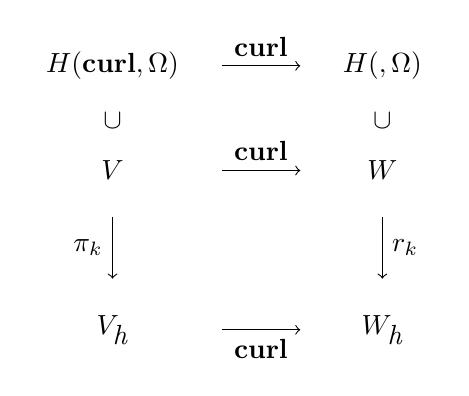
\begin{tikzpicture}[point/.style={circle, inner sep=0pt, minimum size=2pt,fill=red}]
            \matrix[column sep = 1.82mm, row sep = 1.1mm, ampersand replacement = \&] {
             \node {$\text{H}(\textbf{curl},\Omega)$};  
              \& \node (n0) {};
              \& \node      {};
              \& \node (n1) {};
              \& \node (n2) {};
              \& \node {$\text{H}(\Div, \Omega)$}; \\
             \node (n3) {}; \&\&\&\&\& \node (n5)   {}; \\
             \node (n4) {}; \&\&\&\&\& \node (n6)   {}; \\  
             \node (v)  {$V$}; \&\node(fromV){};\&\&\&\node(toW){};\& \node (w) {$W$}; \\
             \node (n7) {}; \&\&\&\&\& \node (n8)   {}; \\ 
             \node      {}; \&\&\&\&\& \node        {}; \\ 
             \node      {}; \&\&\&\&\& \node        {}; \\ 
             \node (n11)    {}; \&\&\&\&\& \node (n12) {}; \\ 
             \node {$V_{\textit{h}} $};                                 
              \& \node (n13) {};
              \& \node       {};
              \& \node (n14) {};
              \& \node (n15) {};
              \& \node (n16) {}; 
             \node {$W_{\textit{h}} $}; \\
             };
            \draw[->] (n0) to node[above] {$\textbf{curl}$} (n2); 
            \draw[->] (fromV) to node[above] {$\textbf{curl}$} (toW); 
            \draw[white] (n3) to node {{\color{black}$\cup$}} (n4);
            \draw[white] (n5) to node {{\color{black}$\cup$}} (n6);
            \draw[->] (n7) to node[left] {$\pi_k$} (n11); 
            \draw[->] (n8) to node[right] {$\boldsymbol{r}_k$} (n12); 
            \draw[->] (n13) to node[below] {$\textbf{curl}$} (n15); 
        \end{tikzpicture}
    \end{center}

% subsection definition_of_the_h_div_element (end)

\subsection{Transformaciones entre prismas} % (fold)
\label{sub:transformaciones_entre_prismas}
Consideremos la aplicación $\hat{\textbf{x}}\longmapsto{\textbf{x}} = 
F_K(\hat{\textbf{x}})$, en donde $F_K = M\hat{\textbf{x}} + \textbf{x}_0$, que transforma
$\hat{K}$ en un elemento $K$ de la malla y $M$ es inversible y tiene determinante 
de signo constante.
Si tenemos una función escalar $\hat{p} \in H^1(\hat{K})$ definimos $p$ en $K$ por
\begin{IEEEeqnarray}{rCl}
    \label{transfEscalar} p\circ F_K & = & \hat{p}.
\end{IEEEeqnarray}
Then, with multiindex notation, for $F_K = \diag{h_1}{h_2}{h_3}$:
\begin{IEEEeqnarray*}{rCl}
    \partial^\alpha \hat{u} (\hat{\textbf{x}})&=&
        h^\alpha\partial^\alpha u(F_K(\hat{\textbf{x}})).
\end{IEEEeqnarray*}
Como $\nabla p = M^{-t}\hat{\nabla} \hat{p} \circ F_K^{-1}$, entonces resulta 
$p \in H^1(K)$.
Ahora tomemos $\hat{\textbf{u}} \in H(curl, \hat{K})$. Buscamos asociarle una
$\textbf{u}$ en $K$. Como para $\hat{p}$ y $p$ como recién vale
$\nabla p \in H(curl, K)$ y $\hat{\nabla} \hat{p} \in H(curl, \hat{K})$, la igualdad
anterior nos sugiere la transformación de $\hat{\textbf{u}}$ a $\textbf{u}$. En efecto
\begin{IEEEeqnarray}{rCl}
    \label{transfHcurl} \textbf{u}\circ F_K & = & M^{-t}\hat{\textbf{u}}.
\end{IEEEeqnarray} 
Con esta definición tenemos $\textbf{u}\in H(\textbf{curl}, K)$ y además
\begin{IEEEeqnarray}{rCl}
    \label{transfCurl} (\textbf{curl}\,\textbf{u})\circ F_K & = & 
    \frac{1}{\det M} M (\hat{\textbf{curl}}\,\hat{\textbf{u}}).
\end{IEEEeqnarray}
Transformación en $H(\dvg)$. Since $F_K$ is affine
\begin{IEEEeqnarray}{rCl}
    \label{transfDiv} \textbf{u}\circ F_K & = & 
    \frac{1}{\det M} M \hat{\textbf{u}}.
\end{IEEEeqnarray}
With~(\ref{transfDiv})
\begin{IEEEeqnarray*}{rCl}
    \|\hat{\textbf{v}}\|^2_{L^2(\hat{K})}
    &=& \sum_{1\leqslant i\leqslant 3}\|\hat{v}_i\|^2_{0,\hat{K}}\\[7pt]
    &=& \sum_{1\leqslant i\leqslant 3}\frac{h_jh_k}{h_i}\,\|v_i\|^2_{0,K};\\[7pt]
    \|\hat{v}_i\|^2_{0,\hat{K}}&=&\frac{h_jh_k}{h_i}\,\|v_i\|^2_{0,K}
\end{IEEEeqnarray*}
where $\{i,j,k\} = \{1,2,3\}$.
\begin{lemma} For all $\tilde{\boldsymbol{\sigma}} \in H(\dvg, \tilde{K})$, $\boldsymbol{\sigma}$ results in
$H(\dvg, K)$ and in fact
\[
    \emph{div}\,\boldsymbol{\sigma}(\emph{\textbf{x}}) =
        \frac{1}{\det DF}\,\tilde{\emph{div}}\,\tilde{\boldsymbol{\sigma}}(\tilde{\emph{\textbf{x}}}).
\]
\end{lemma}
\begin{proof}
Observe that
\begin{IEEEeqnarray*}{rCl}
    trace(A\cdot B\cdot A^{-1}) &=& trace(B)\\
    \label{Piola}\yesnumber\boldsymbol{\sigma} \circ F & = & \frac{1}{\det(A)} A\,\tilde{\boldsymbol{\sigma}}\\
    \label{derivadaPiola}\yesnumber\tilde{D}\tilde{\boldsymbol{\sigma}}(\tilde{\textbf{x}}) & = &
        \det(A)\,A^{-1}\,D\boldsymbol{\sigma} (F(\tilde{\textbf{x}})) \,A.
\end{IEEEeqnarray*}
Then
\begin{IEEEeqnarray*}{rCl}
    \text{div}\,\boldsymbol{\sigma}(\textbf{x}) & = & trace(D\boldsymbol{\sigma} (\textbf{x}))\\
                                        & = & \frac{1}{\det(A)}\,trace(A\,\tilde{D}\tilde{\boldsymbol{\sigma}} (F^{-1}(\textbf{x}))\,A^{-1})\\
                                        & = & \frac{1}{\det(A)}\,\tilde{\text{div}}\,\tilde{\boldsymbol{\sigma}}(\tilde{\textbf{x}}).   
\end{IEEEeqnarray*}
\end{proof}

Todas estas igualdades se prueban en~\cite{monk}.\\\\
Citar de~\cite{monk}. 
\begin{lemma} The edge element interpolators satisfy
\begin{IEEEeqnarray}{rCl}\label{piTransformado}
    \hat{\pi}_k(\hat{\textbf{u}})(\hat{\textbf{x}}) & = & M^{t} \pi_k(\textbf{u})(\textbf{x}).
\end{IEEEeqnarray}
{\color{BrickRed} > lo probamos?}
\end{lemma}

% subsection transformaciones_entre_prismas (end)